\section{Modelagem no espa�o das juntas}
Manipuladores subatuados diferem dos totalmente atuados pois s�o equipados com um n�mero de atuadores que � sempre menor que o n�mero de graus de liberdade (GDL). Portanto, nem todos os GDL podem ser controlados ativamente ao mesmo tempo \cite{Sbornian2004}. Por exemplo, com um manipulador planar de 3 juntas equipado com dois atuadores, ou seja, duas juntas ativas e
uma passiva, pode-se controlar ao mesmo tempo duas das juntas a qualquer instante, mas n�o todas. Para controlar todas as juntas de um manipulador subatuado, deve-se usar um controle sequencial. Este princ�pio foi provado pela primeira vez por {arai} usando  argumentos din�micos linearizados \cite{Joea2003}, e � a base para a modelagem no espa�o das juntas e no espa�o Cartesiano. A Tabela \ref{minhatab} apresenta os resultados \cite{Assenmacher1993,Silberschatz1991,Caromel1998}.

\begin{table}
\caption{Exemplo de uma Tabela}
\label{minhatab}

\center
\begin{tabular}{cccc}
  % after \\: \hline or \cline{col1-col2} \cline{col3-col4} ...
  \hline
	Par�metro & Unidade & Valor da simula��o & Valor experimental   \\
	\hline
  Comprimento, $\alpha$ & $m$ &  $8,23$  & $8,54$ \\
  Altura, $\beta$ & $m$     &  $29,1$ & $28,3$\\
	Velocidade, $v$ & $m/s$  &  $60,2$ & $67,3$\\
	\hline
\end{tabular}
\end{table}

Devido ao fato de que no m�ximo $n_{a}$ coordenadas generalizadas (�ngulos das juntas ou vari�veis cartesianas) podem ser controladas num dado instante, o vetor de coordenadas generalizadas � dividido em duas partes, representando as coordenadas generalizadas ativas e as coordenadas generalizadas passivas \cite{Callaghan1995}.

\begin{figure}[ht]
\centering
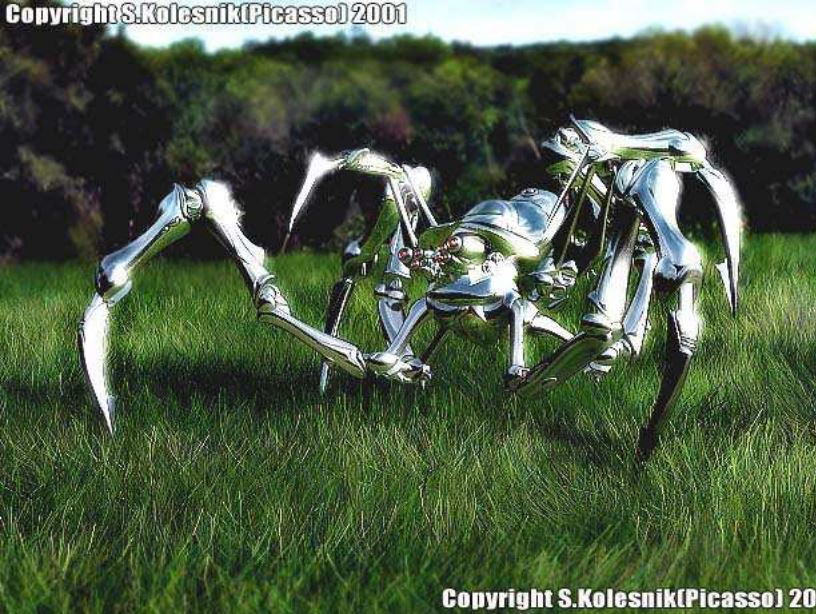
\includegraphics[width=0.75\textwidth]{Cap2/spiderrobot}
\caption{Cupim cibern�tico.}\label{FDIII}
\end{figure}

Considerando um rob� manipulador r�gido, malha aberta, e de $n$-juntas em s�rie. Seja $q$ a representa��o de seu vetor de posi��o angular das juntas  e $\tau$ a representa��o de seu vetor de torque. A equa��o din�mica pelo m�todo de
Lagrange � dada por:
\begin{equation} \label{eq:lagr1}
\frac{d}{dt}(\frac{\partial L}{\partial \dot{q}})-\frac{\partial L}{\partial q}=\tau^{T}.
\end{equation}
O Lagrangiano $L$ � definido como a diferen�a entre as energias cin�tica e potencial do sistema:
\begin{equation} \label{L}
L=T-P
\end{equation}

A energia cin�tica total dos ligamentos � representada:
\begin{equation} \label{energT}
T=\frac{1}{2}\dot{q}^{T}M(q)\dot{q}
\end{equation}
